
Avec $n = 2$, nous avons une façon originale de faire le produit de deux entiers à deux chiffres. Considérons par exemple le produit $56 \cdot 78$. Voici ce que donne la méthode de Karatsuba dans ce cas.
	
\begin{enumerate}
	\item Ici $a = 5$ , $b = 6$ , $A = 7$ et $B = 8$ .

	\item $c_2 = 5 \cdot 7 = 35$ .

	\item $c_0 = 6 \cdot 8 = 48$ .

	\item $c_1 = (5 + 6) \, (7 + 8) - 35 - 48 = 165 - 35 - 48 = 82$ .

	\item $56 \cdot 78 = c_2 \cdot 10^2 + c_1 \cdot 10^1 + c_0 = 3500 + 820 + 48 = 4368$ .
\end{enumerate}
	
\medskip
	
Visuellement nous avons fait les calculs suivants où $c_0$ et $c_2$ sont des multiplications \og verticales \fg{} et $c_1$ s'obtient en soustrayant ces deux multiplications au produit des \og additions horizontales \fg{}.
	
\begin{center}
	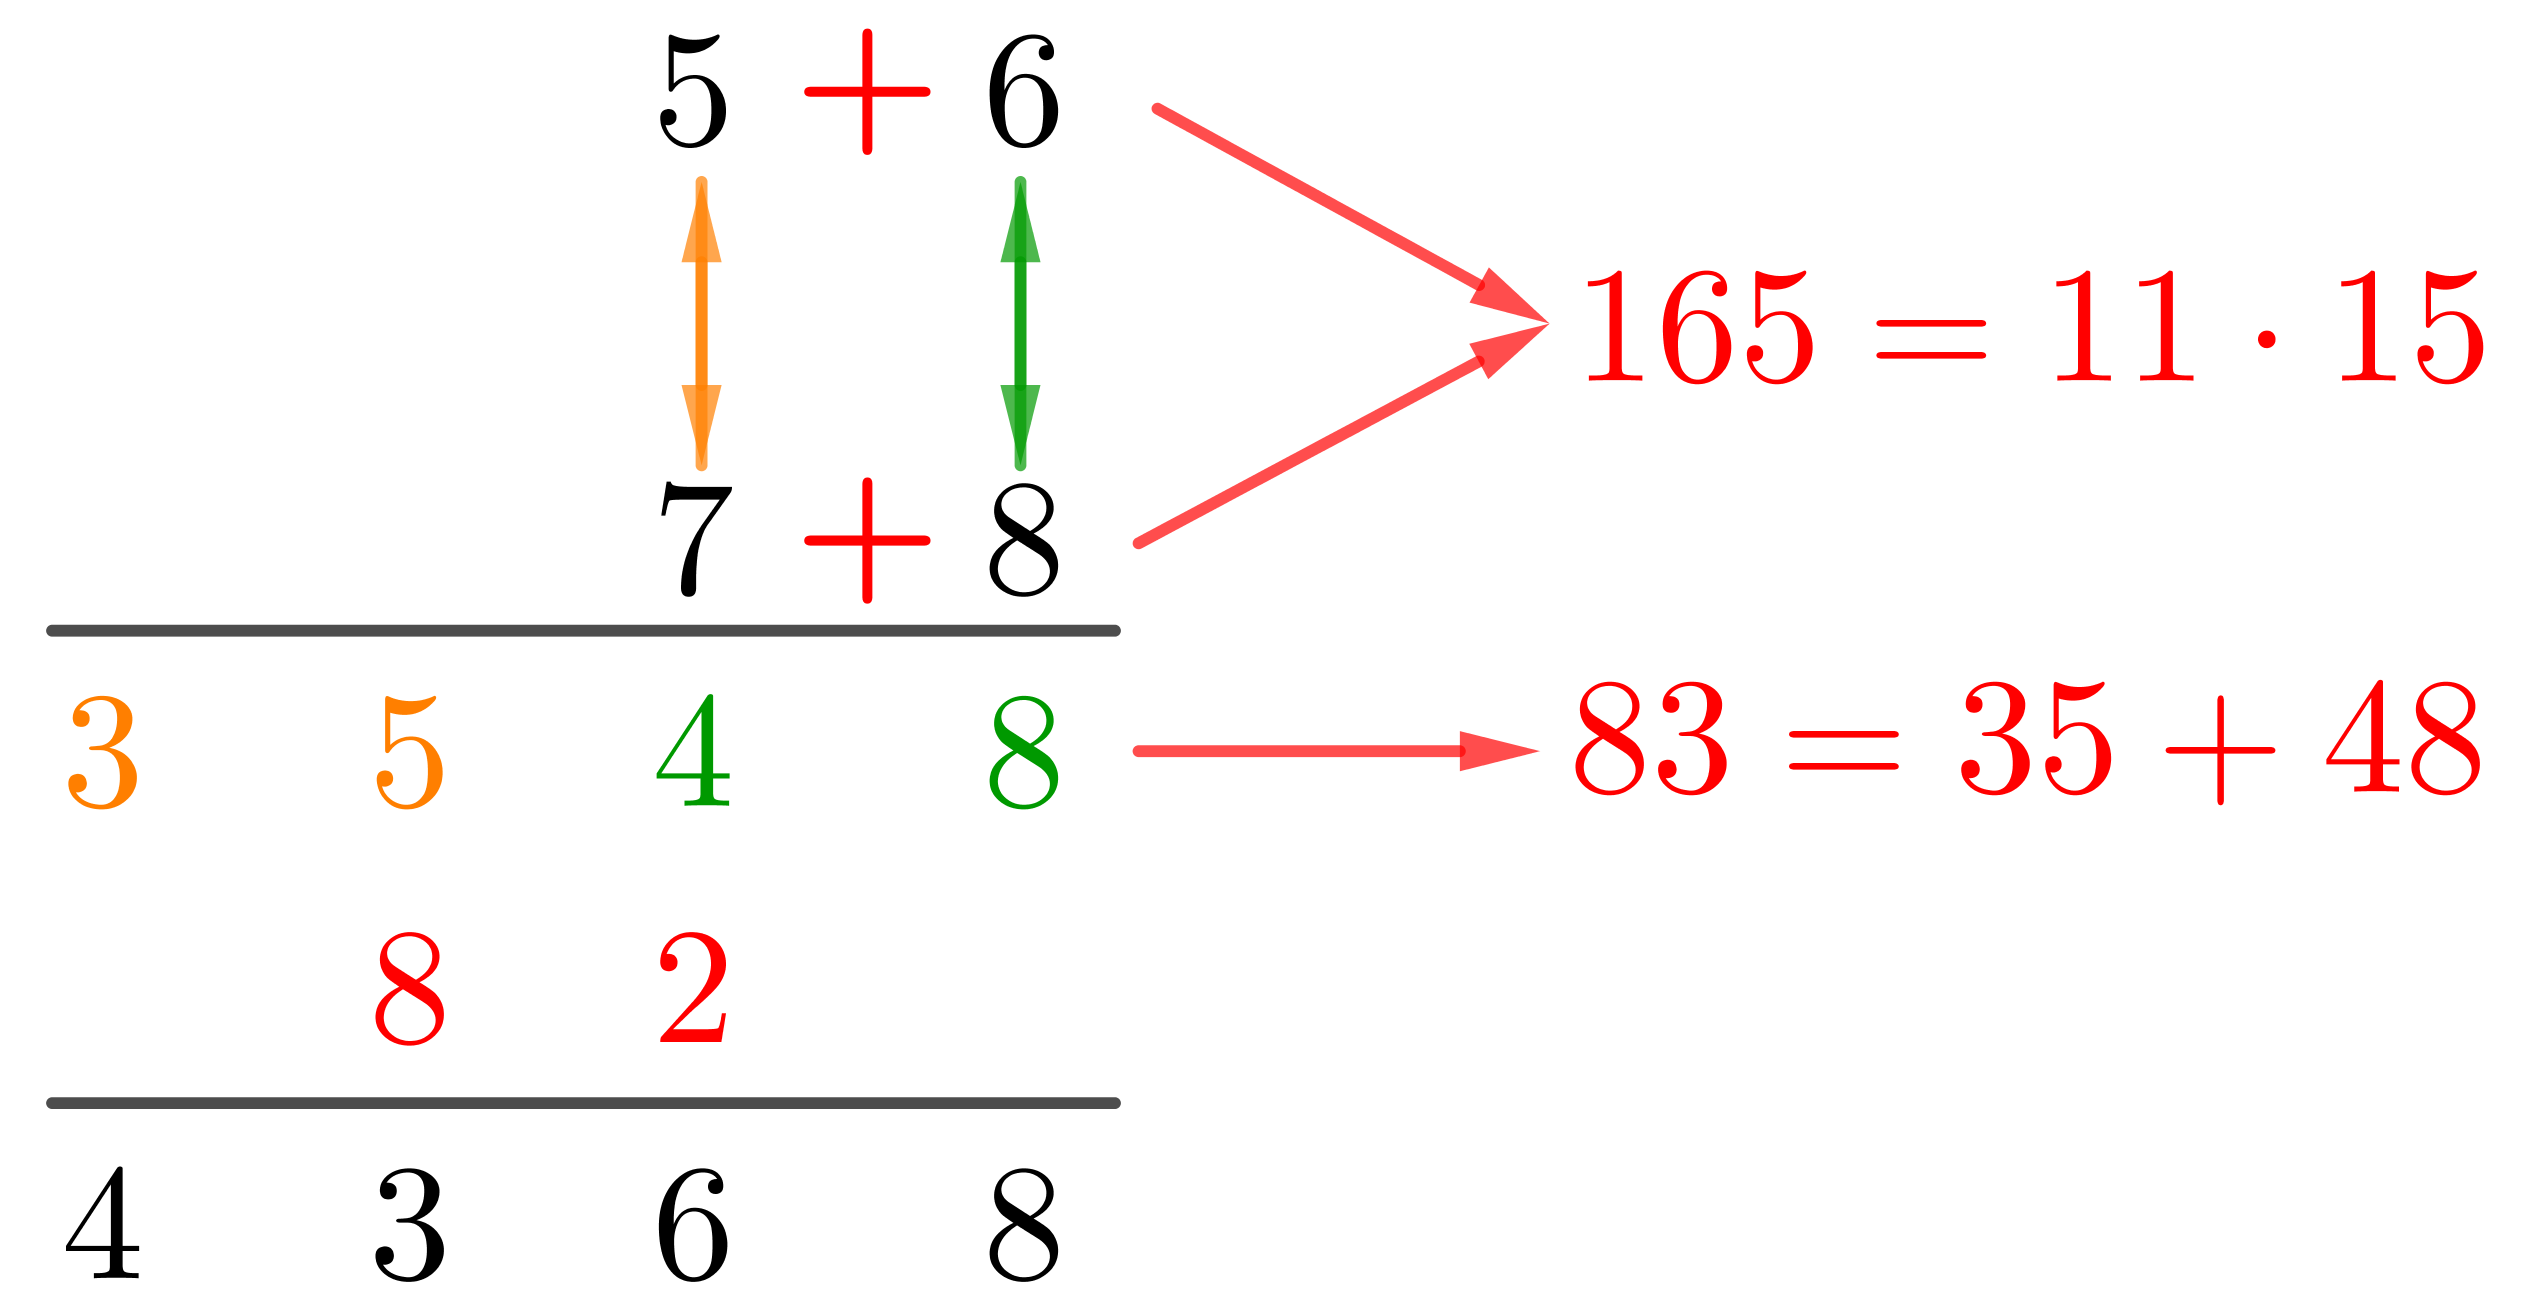
\includegraphics[scale=.75]{not-so-basic-arithmetic-ope/product-two-digits-karatsuba.png}
\end{center}

\medskip

Notons que le calcul directement via
$a \cdot A \cdot 10^2 + (a \cdot B + A \cdot b) \cdot 10 + b \cdot B$
donne une méthode plus utile pour un calcul mental sans crayon ni papier car les calculs se font au fil de l'eau de la droite vers la gauche avec peu de calculs intermédiaires à retenir.
	
\begin{center}
	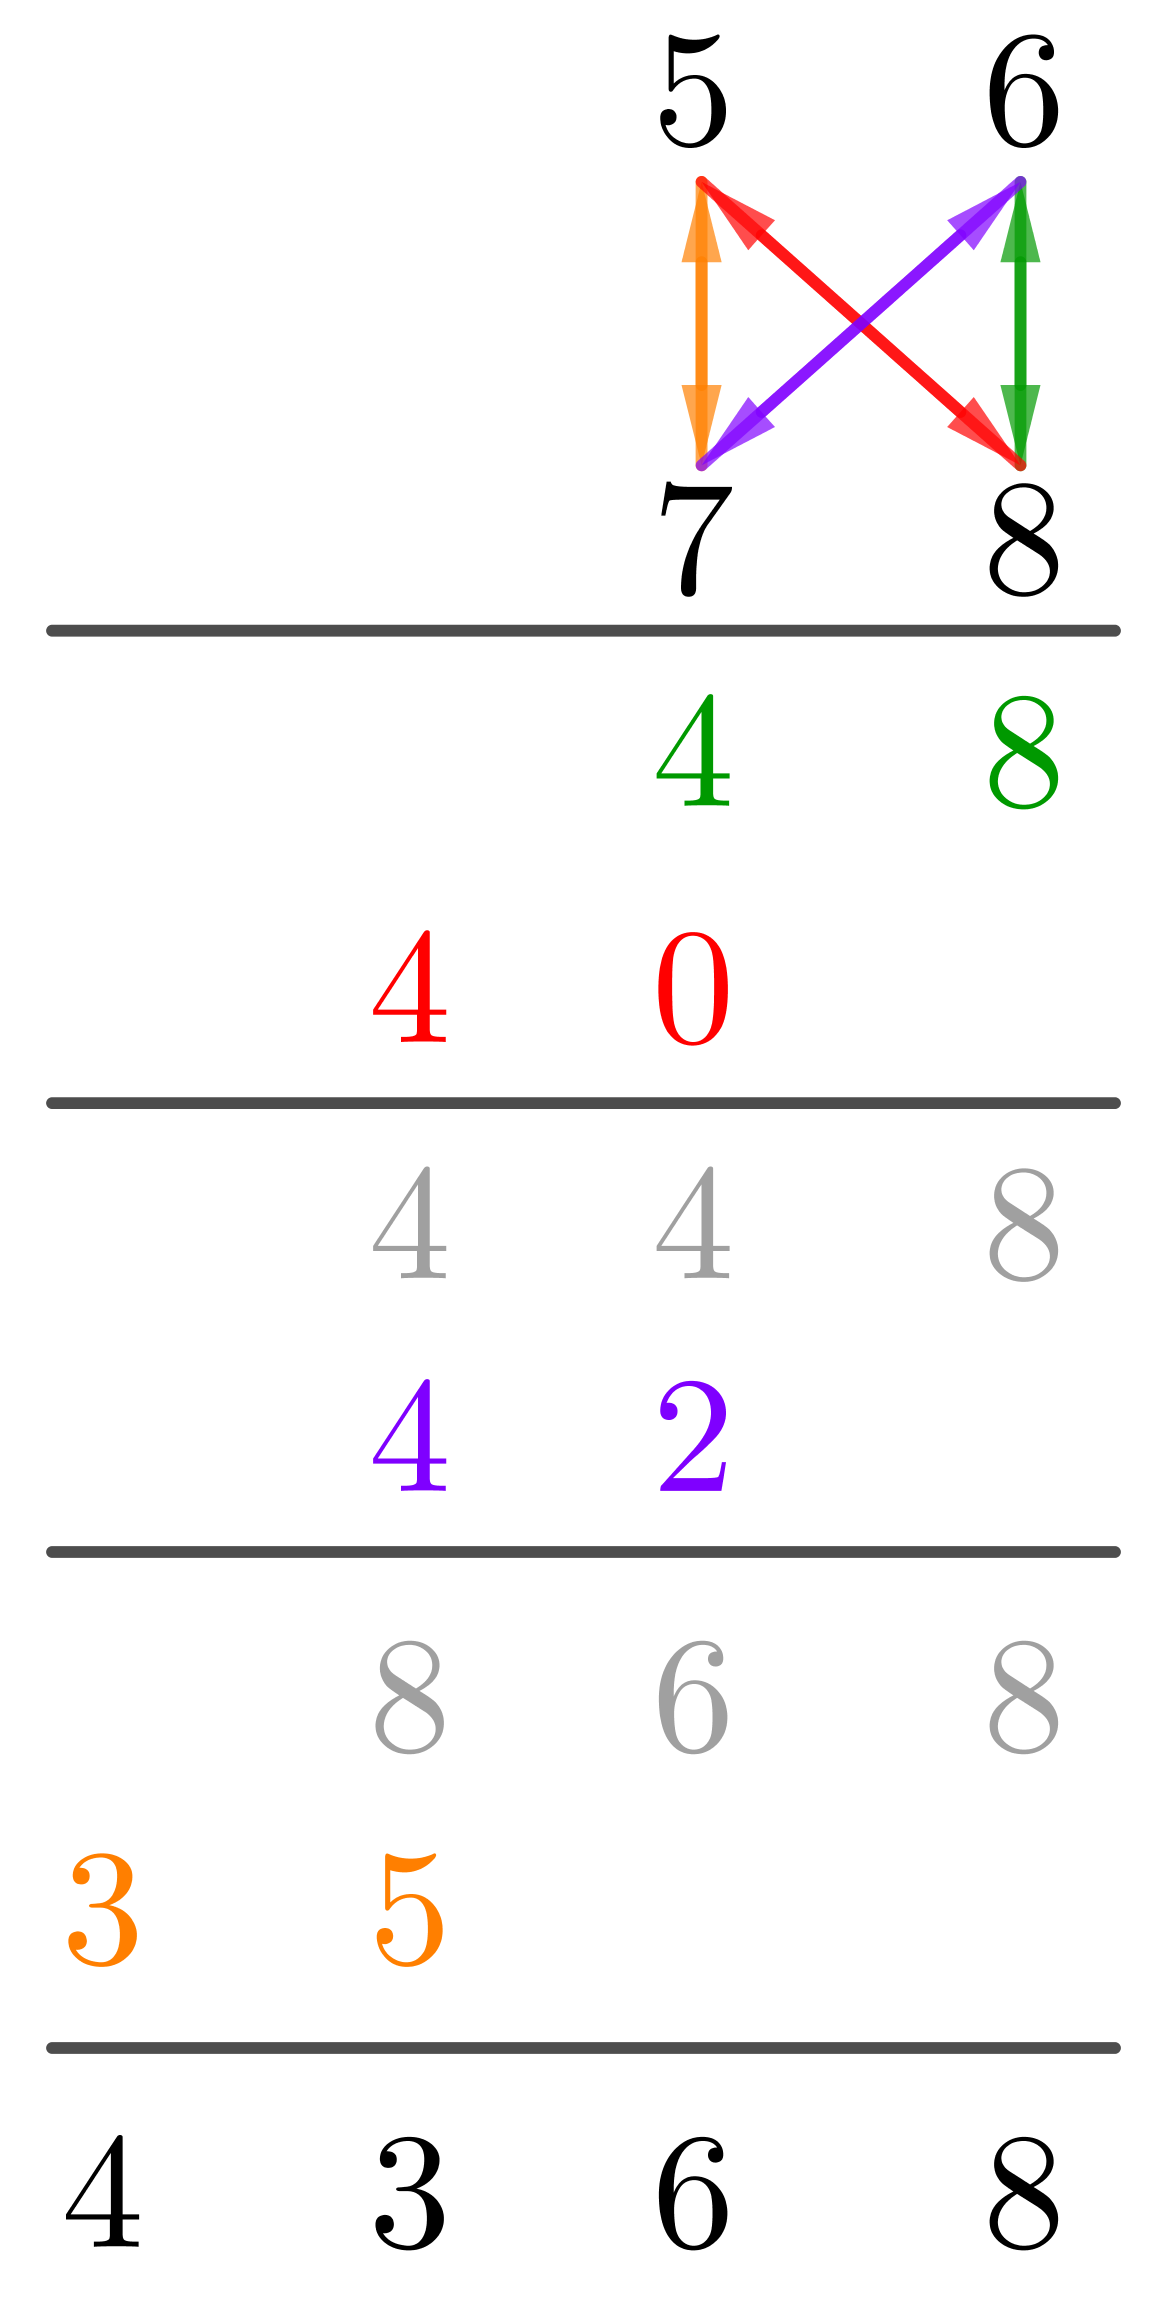
\includegraphics[scale=.75]{not-so-basic-arithmetic-ope/product-two-digits-easier.png}
\end{center}